\documentclass[tikz,border=5pt]{standalone}
\usepackage[T1]{fontenc}
\usepackage{lmodern,amsmath,amssymb}
\usetikzlibrary{arrows.meta,calc,positioning,fit,backgrounds,shapes.geometric,matrix,decorations.pathreplacing,patterns}
\definecolor{ink}{gray}{0.08}
\definecolor{wash}{gray}{0.965}
\definecolor{soft}{gray}{0.45}
\tikzset{box/.style={draw=ink,line width=.65pt,fill=white,align=center,inner sep=4pt,outer sep=0pt,font=\small},flow/.style={draw=ink,line width=.65pt,-{Latex[length=1.8mm,width=1.3mm]},rounded corners=2pt},annotation/.style={font=\scriptsize,text=soft,align=center},groupbox/.style={draw=soft,dashed,line width=.45pt,fill=wash}}
\begin{document}
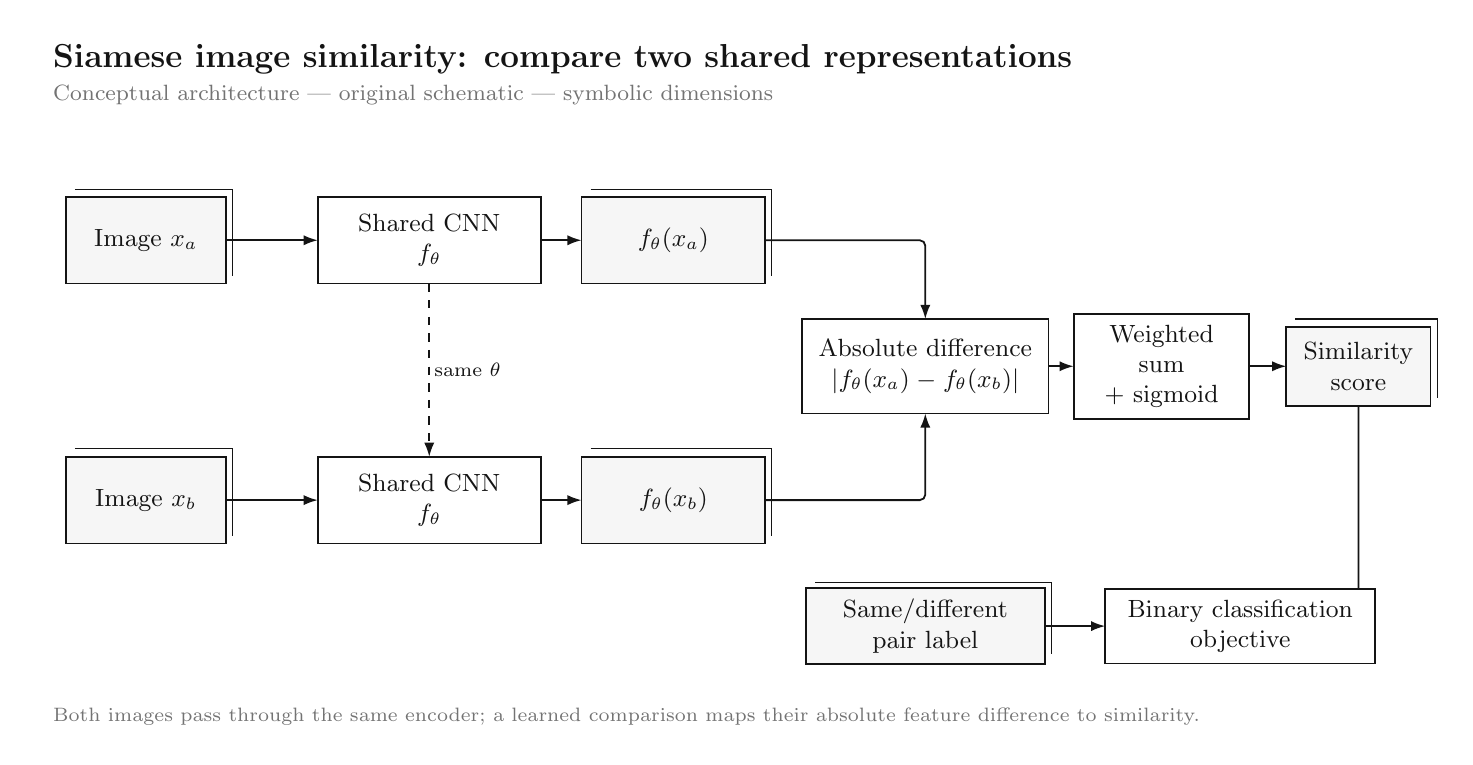
\begin{tikzpicture}[x=1cm,y=-1cm,font=\rmfamily,text=ink]

\path[use as bounding box] (0,0) rectangle (18,9);
\node[anchor=west,font=\large\bfseries] at (.2,.4) {Siamese image similarity: compare two shared representations};
\node[anchor=west,font=\footnotesize,text=soft] at (.2,.85) {Conceptual architecture | original schematic | symbolic dimensions};
\begin{pgfonlayer}{background}
\end{pgfonlayer}
\node[box,fill=wash,minimum width=2.0cm,minimum height=1.1cm,text width=1.75cm] (xa) at (1.5,2.7) {Image $x_a$};
\draw[ink,line width=.4pt] (0.6,2.0500000000000003) -- (2.6,2.0500000000000003) -- (2.6,3.15);
\node[box,minimum width=2.8cm,minimum height=1.1cm,text width=2.55cm] (fa) at (5.1,2.7) {Shared CNN\\$f_\theta$};
\node[box,fill=wash,minimum width=2.3cm,minimum height=1.1cm,text width=2.05cm] (ea) at (8.2,2.7) {$f_\theta(x_a)$};
\draw[ink,line width=.4pt] (7.149999999999999,2.0500000000000003) -- (9.45,2.0500000000000003) -- (9.45,3.15);
\node[box,fill=wash,minimum width=2.0cm,minimum height=1.1cm,text width=1.75cm] (xb) at (1.5,6.0) {Image $x_b$};
\draw[ink,line width=.4pt] (0.6,5.3500000000000005) -- (2.6,5.3500000000000005) -- (2.6,6.45);
\node[box,minimum width=2.8cm,minimum height=1.1cm,text width=2.55cm] (fb) at (5.1,6.0) {Shared CNN\\$f_\theta$};
\node[box,fill=wash,minimum width=2.3cm,minimum height=1.1cm,text width=2.05cm] (eb) at (8.2,6.0) {$f_\theta(x_b)$};
\draw[ink,line width=.4pt] (7.149999999999999,5.3500000000000005) -- (9.45,5.3500000000000005) -- (9.45,6.45);
\node[box,minimum width=3.1cm,minimum height=1.2cm,text width=2.85cm] (diff) at (11.4,4.3) {Absolute difference\\$|f_\theta(x_a)-f_\theta(x_b)|$};
\node[box,minimum width=2.2cm,minimum height=1.1cm,text width=1.9500000000000002cm] (cmp) at (14.4,4.3) {Weighted sum\\+ sigmoid};
\node[box,fill=wash,minimum width=1.8cm,minimum height=1.0cm,text width=1.55cm] (score) at (16.9,4.3) {Similarity\\score};
\draw[ink,line width=.4pt] (16.099999999999998,3.6999999999999997) -- (17.9,3.6999999999999997) -- (17.9,4.7);
\node[box,fill=wash,minimum width=3.0cm,minimum height=0.9cm,text width=2.75cm] (pair) at (11.4,7.6) {Same/different\\pair label};
\draw[ink,line width=.4pt] (10.0,7.05) -- (13.0,7.05) -- (13.0,7.949999999999999);
\node[box,minimum width=3.4cm,minimum height=0.9cm,text width=3.15cm] (loss) at (15.4,7.6) {Binary classification\\objective};
\begin{pgfonlayer}{background}
\draw[flow] (xa.east) -- (fa.west);
\draw[flow] (fa.east) -- (ea.west);
\draw[flow] (xb.east) -- (fb.west);
\draw[flow] (fb.east) -- (eb.west);
\draw[flow,dashed] (fa.south) -- (fb.north) node[midway,right,fill=white,inner sep=1.5pt,font=\scriptsize] {same $\theta$};
\draw[flow] (ea.east) -- (11.4,2.7) -- (diff.north);
\draw[flow] (eb.east) -- (11.4,6.0) -- (diff.south);
\draw[flow] (diff.east) -- (cmp.west);
\draw[flow] (cmp.east) -- (score.west);
\draw[flow] (pair.east) -- (loss.west);
\draw[flow] (score.south) -- (16.9,7.6) -- (loss.east);
\end{pgfonlayer}
\node[anchor=west,align=left,font=\scriptsize,text=soft,text width=17.6cm] at (.2,8.75) {Both images pass through the same encoder; a learned comparison maps their absolute feature difference to similarity.};
\end{tikzpicture}
\end{document}
